\chapter{Research Methodology}

\section{Research Design}

This research adopts a system development and experimental approach to implement and validate a proactive forensic framework for online examination systems. The proposed framework adheres to the structured log management principles outlined in the NIST SP 800-92 standard~\cite{kentnist800922006guide}, aiming to establish a centralized, secure, and automated environment for collecting, analyzing, and preserving digital evidence.

The system is integrated with a Moodle-based Learning Management System (LMS), simulating an English Proficiency Test (EPT). Log data from quiz attempts and participant activities are systematically collected and analyzed using machine learning-based anomaly detection. Key features of the system include real-time monitoring, a web-based dashboard, and alert mechanisms to enhance forensic readiness.

\subsection{System Implementation}

The proactive forensic system includes a log acquisition stage using automated scripts to extract daily activity data. This data is stored in a designated log repository and analyzed using machine learning to detect anomalies. A dashboard web application is developed to visualize log activities and notify stakeholders of suspicious events via Telegram bot integration.

The system architecture is modeled after the existing infrastructure of a university’s online examination environment, using Moodle LMS and Azure-based virtual machines. Figure~\ref{fig:lms-architecture} illustrates the reference architecture, while Figure~\ref{fig:vmss-architecture} depicts the use of Azure Virtual Machine Scale Sets (VMSS) to ensure scalability.

\begin{figure}[H]
    \centering
    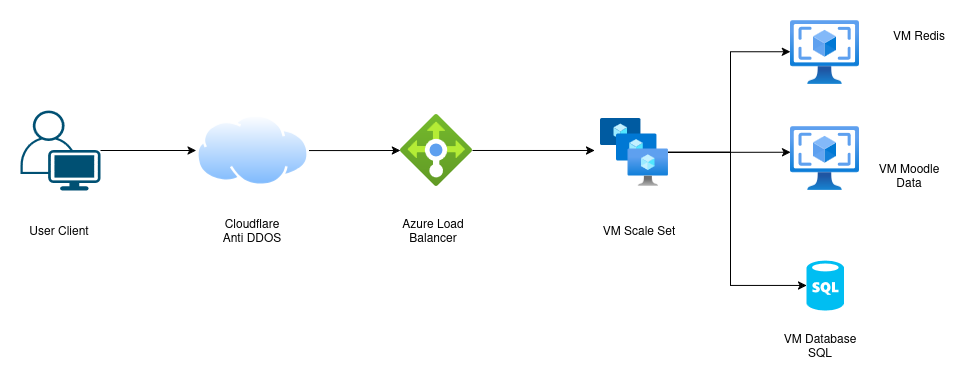
\includegraphics[width=14cm]{figure/architecture-lac-architecture LAC level 1.drawio.png}
    \caption{Reference architecture of the university’s online examination system}
    \label{fig:lms-architecture}
\end{figure}

\begin{figure}[H]
    \centering
    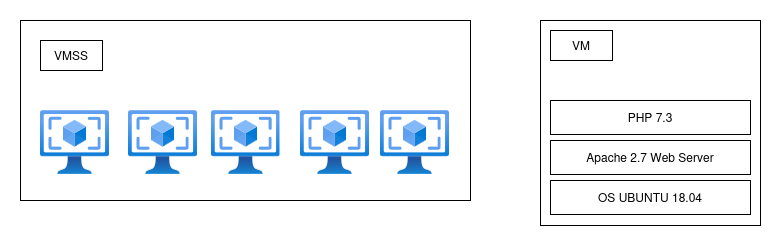
\includegraphics[width=14cm]{figure/vmss.drawio.png}
    \caption{Architecture of Azure VM Scale Set used in the implementation}
    \label{fig:vmss-architecture}
\end{figure}

The system infrastructure utilizes a Virtual Machine Scale Set (VMSS) to dynamically manage computing resources during online examinations. VMSS enables automatic provisioning (\textit{auto-create}) of virtual machines when an exam session begins, and de-provisioning (\textit{auto-destroy}) once the session has ended. 

% \subsection{Research Phases Plan}

% \begin{figure}[H]
%     \centering
%     
\includegraphics[width=14cm]{figure/research-phase.png}
%     \caption{Research Phase}
%     \label{fig:research-phase}
% \end{figure}

% \begin{table}[H]
% \centering
% \caption{Development Phases and Activities}
% \label{tab:phase-method}
% \begin{tabular}{@{}p{3cm}p{7cm}p{4cm}@{}}
% \toprule
% \textbf{Phase} & \textbf{Activity} & \textbf{Outcome} \\
% \midrule
% Planning & Identify goals and gather system requirements & Clearly defined objectives \\
% Analysis & Identify log sources and data structure & Detailed analysis documentation \\
% Design & Develop system architecture and build prototype & System blueprint and design artifacts \\
% Implementation & Code development and system integration & Functional prototype \\
% Testing & System functionality and component verification & Validated and verified framework \\
% \bottomrule
% \end{tabular}
% \end{table}

% Table~\ref{tab:phase-method} presents the sequential phases involved in the system development, including planning, analysis, design, implementation, and testing.

\begin{figure}[H]
    \centering
    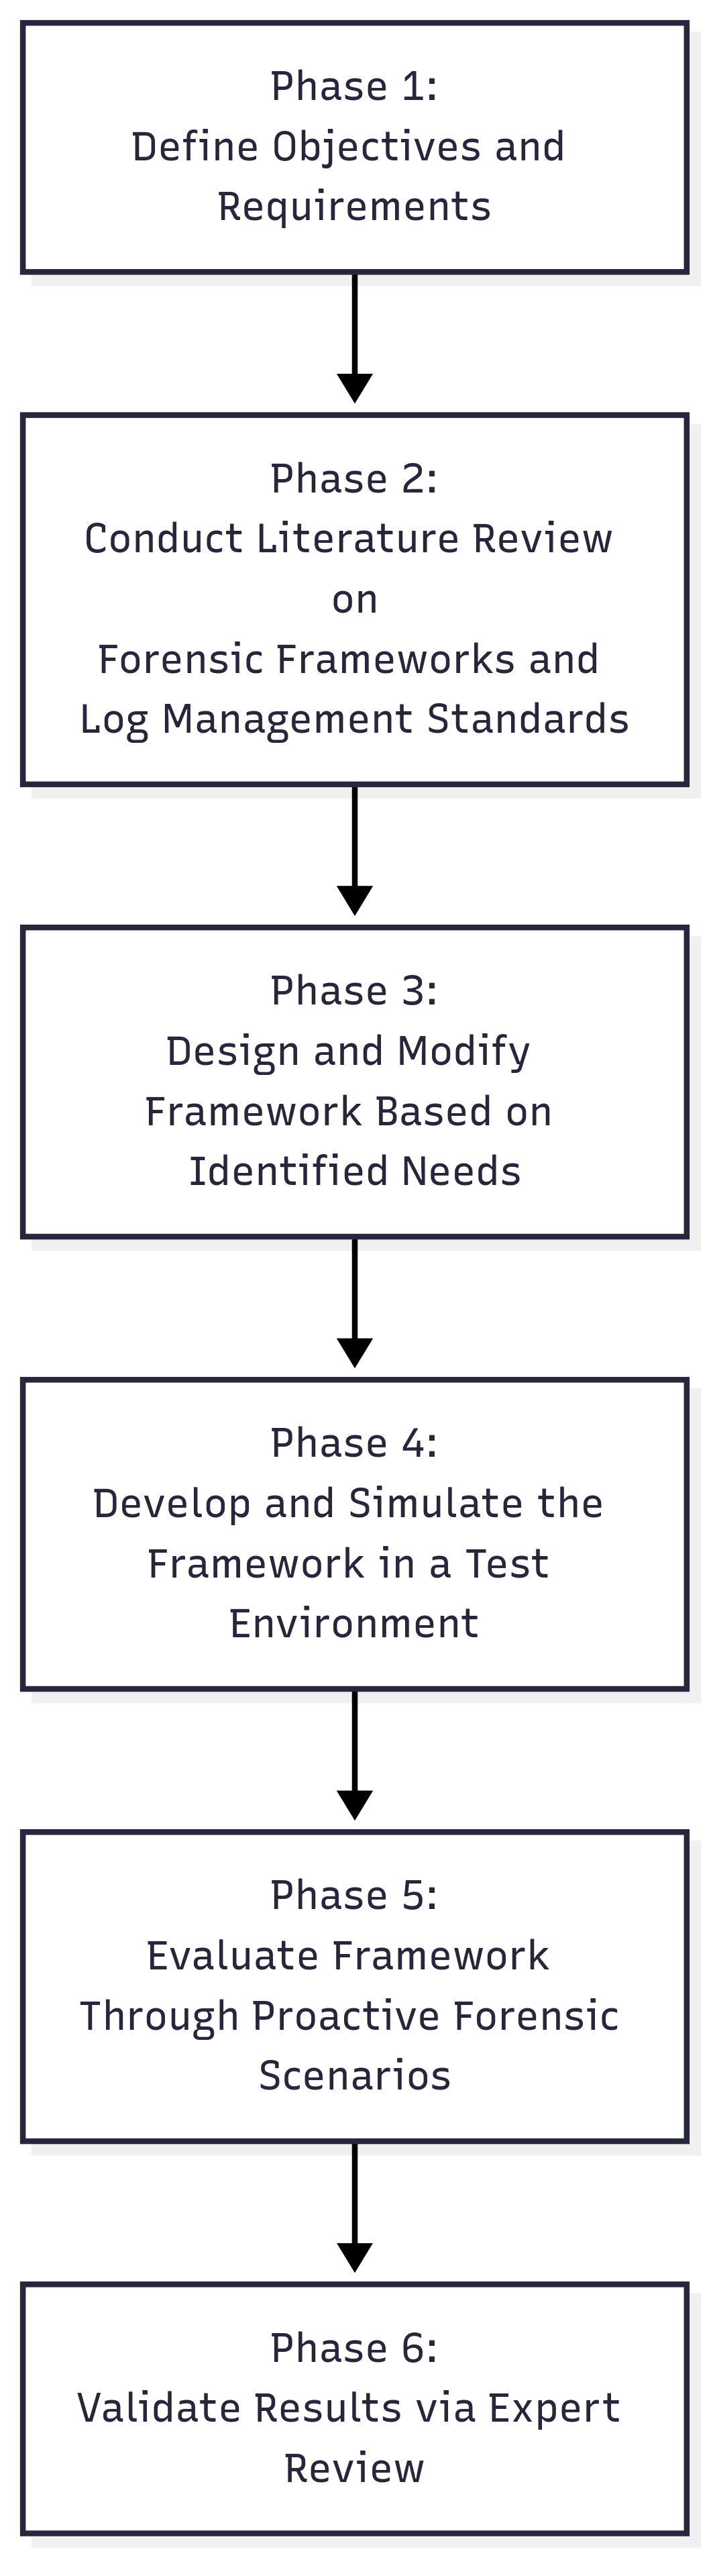
\includegraphics[width=8cm,height=19cm]{figure/framework-development.png}
    \caption{Proactive Forensic Framework Development Phase \citet{adel2024ethicore}}
    \label{fig:framework-development-phase}
\end{figure}
Figure~\ref{fig:framework-development-phase} presents the proposed framework development flow, adapted from Adel et al.~\cite{adel2024ethicore}. The framework consists of six phases: defining objectives, literature review, framework design, simulation, testing, and expert validation. 

The last two phases testing and validation were added to evaluate the framework in real exam scenarios and to gather feedback from domain experts in digital forensics and educational systems. This ensures both technical reliability and practical relevance in online examination contexts.

\begin{table}[H]
\centering
\caption{Stages of Framework Development}
\begin{tabular}{|c|p{4.5cm}|p{8.5cm}|}
\hline
\textbf{No.} & \textbf{Stage} & \textbf{Description} \\
\hline
1 & Define Objectives and Requirements & Identify the primary goals and specific requirements for developing the forensic log management framework. \\
\hline
2 & Conduct Literature Review on Forensic Frameworks and Log Management Standards & Study existing research, models, and relevant standards (e.g., NIST SP 800-92) to gain insight and identify gaps. \\
\hline
3 & Design and Modify Framework Based on Identified Needs & Create or adapt framework components to match the defined objectives and contextual system needs. \\
\hline
4 & Develop and Simulate the Framework in a Test Environment & Implement the proposed framework in a controlled testbed to observe log flow and system behavior. \\
\hline
5 & Evaluate Framework Through Proactive Forensic Scenarios & Test the framework’s effectiveness by applying it to simulated forensic incidents or attack scenarios. \\
\hline
6 & Validate Results via Expert Review & Review and validate the framework through expert evaluation or feedback for reliability and improvement. \\
\hline
\end{tabular}
\end{table}

Based on the framework development approach proposed by \citet{adel2024ethicore}, this research follows a structured process that begins with identifying existing forensic frameworks and relevant standards. The framework is then designed to address specific needs in digital forensics for online examination environments. To ensure that the framework is practical and effective, it is evaluated through scenario-based testing that simulates real forensic cases in online exams. Finally, validation is conducted by consulting experts in the field, including digital forensic professionals and education technology specialists, to assess the relevance, completeness, and applicability of the framework in real-world settings.

\begin{figure}[H]
    \centering
    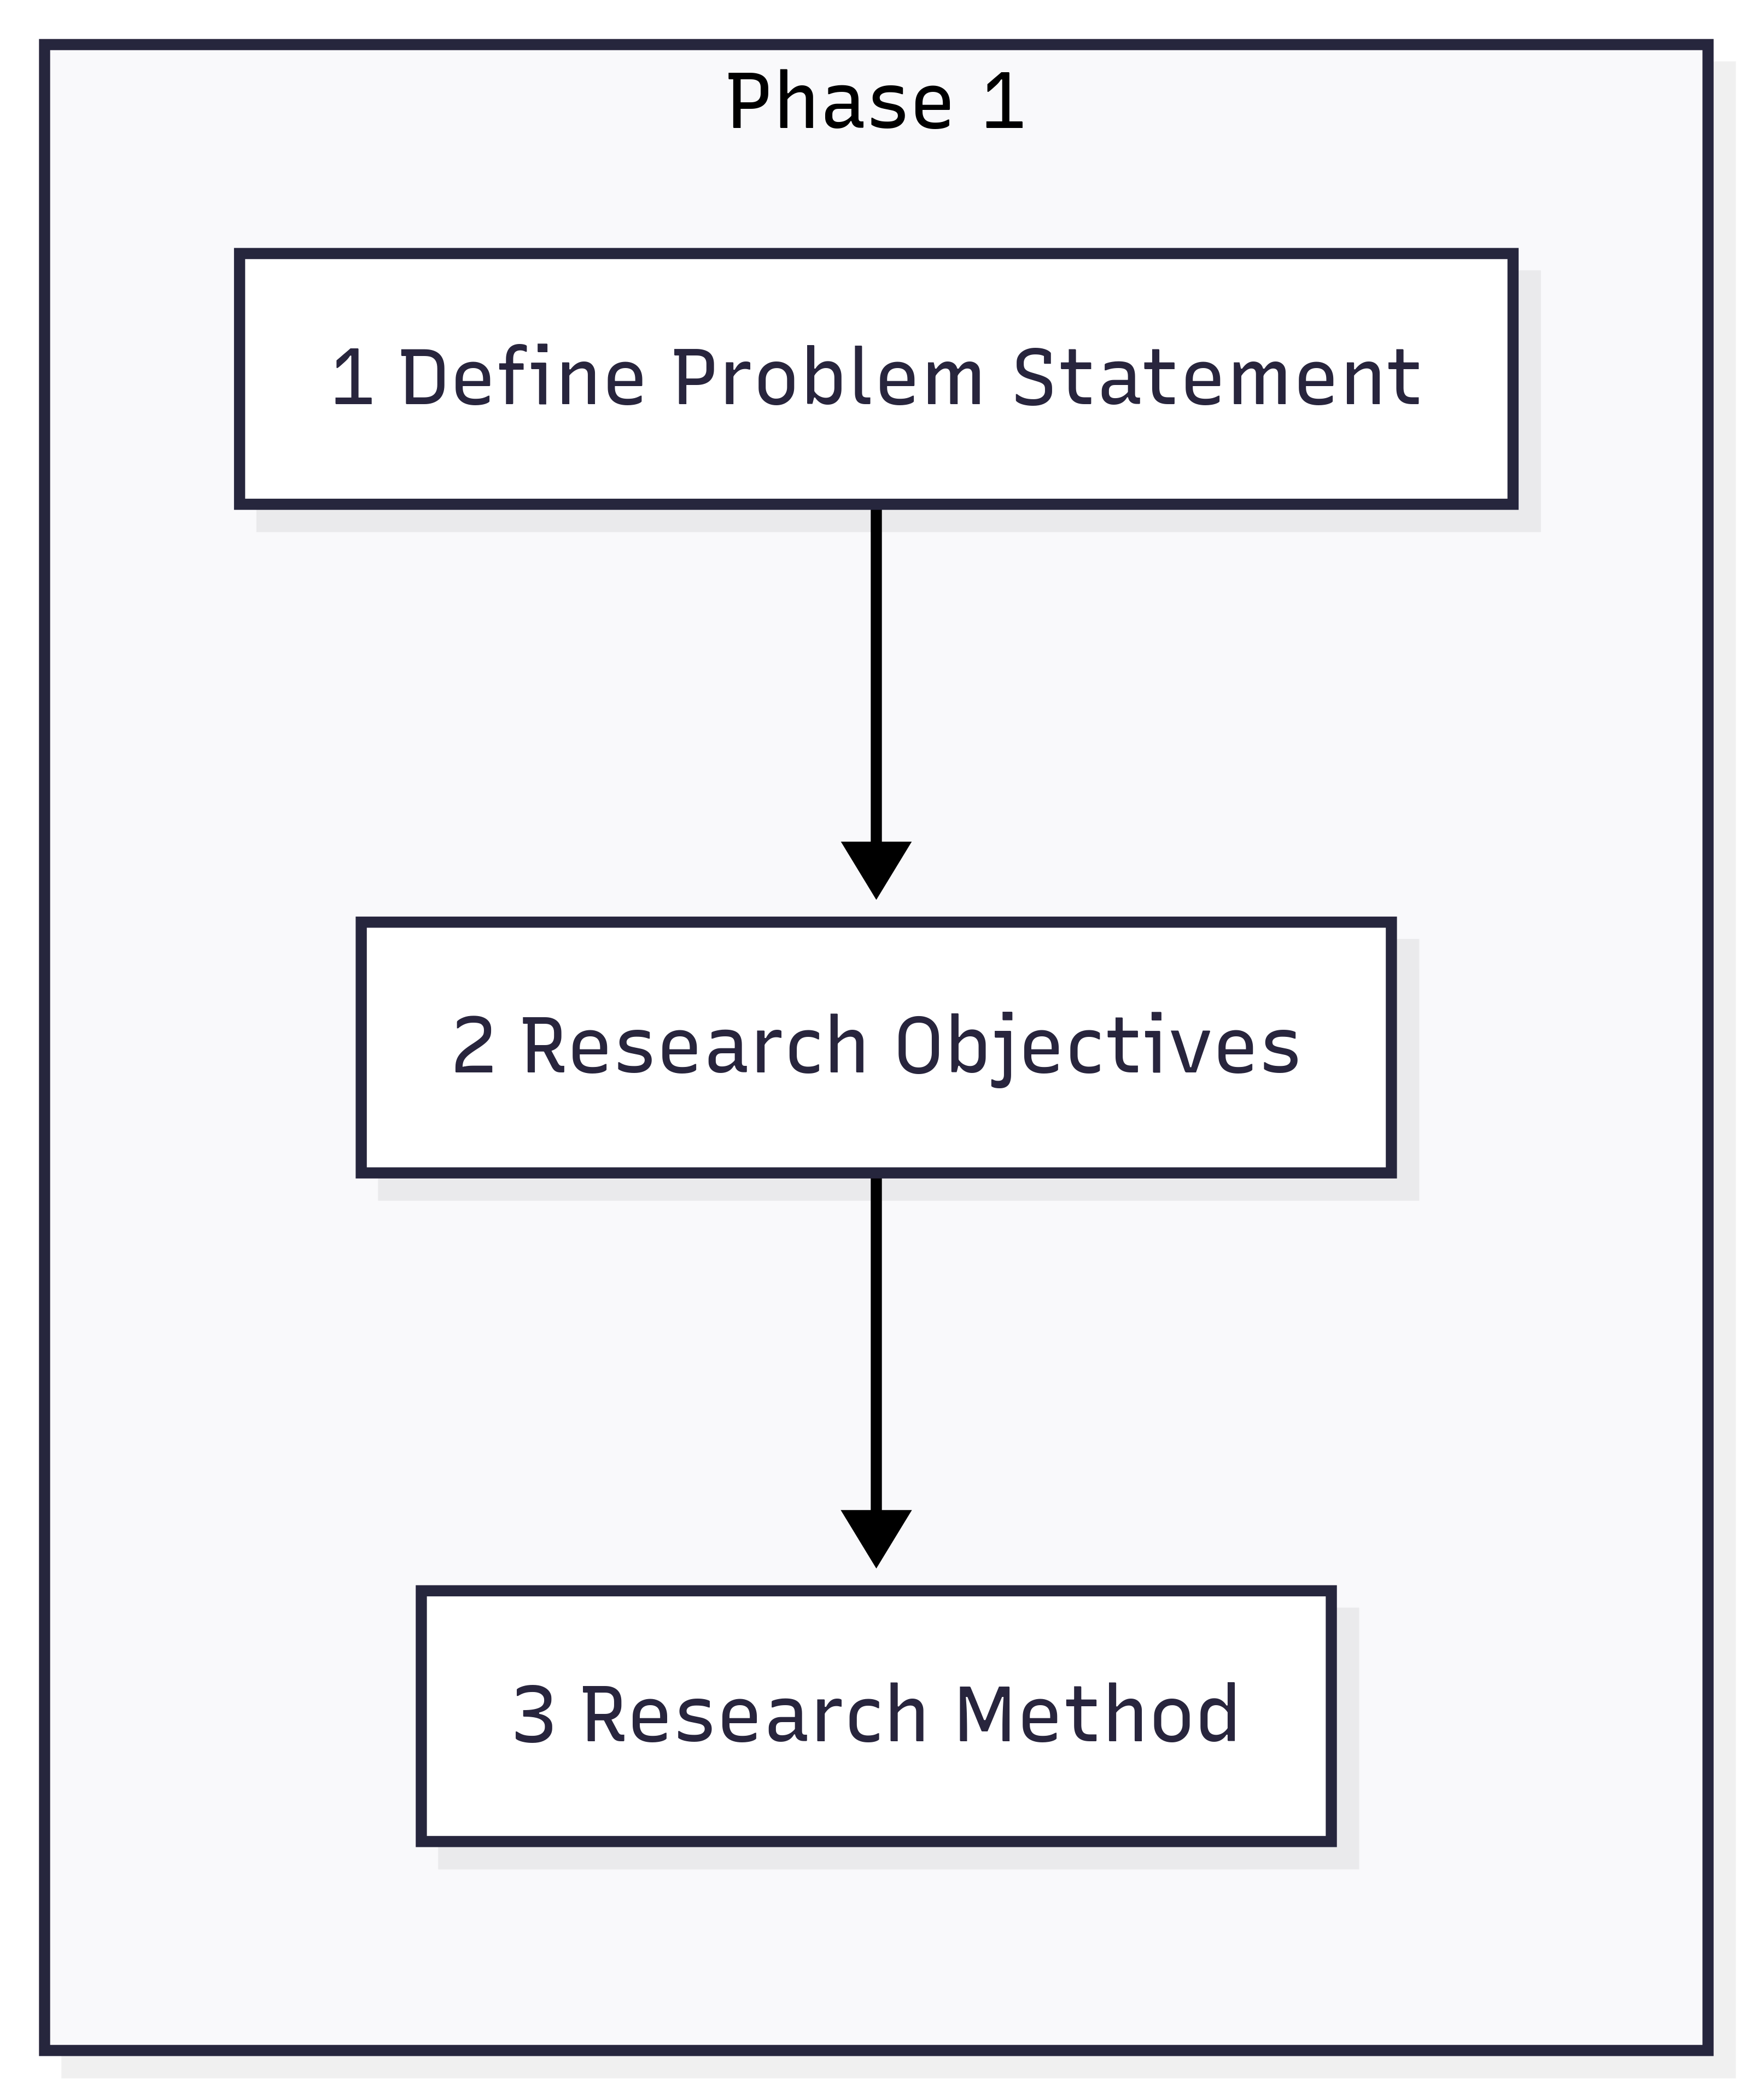
\includegraphics[height=14cm]{figure/framework-development-phase-1.png}
    \caption{Proactive Forensic Framework Development Phase 1}
    \label{fig:framework-development-phase-1}
\end{figure}

As shown in Figure~\ref{fig:framework-development-phase-1}, the first phase focuses on understanding the problem domain by identifying the challenges associated with digital forensic investigations in online learning systems. This phase includes formulating the problem statement, defining research objectives, and selecting appropriate research methods. The output of this phase forms the foundation for all subsequent design and development activities.


\begin{figure}[H]
    \centering
    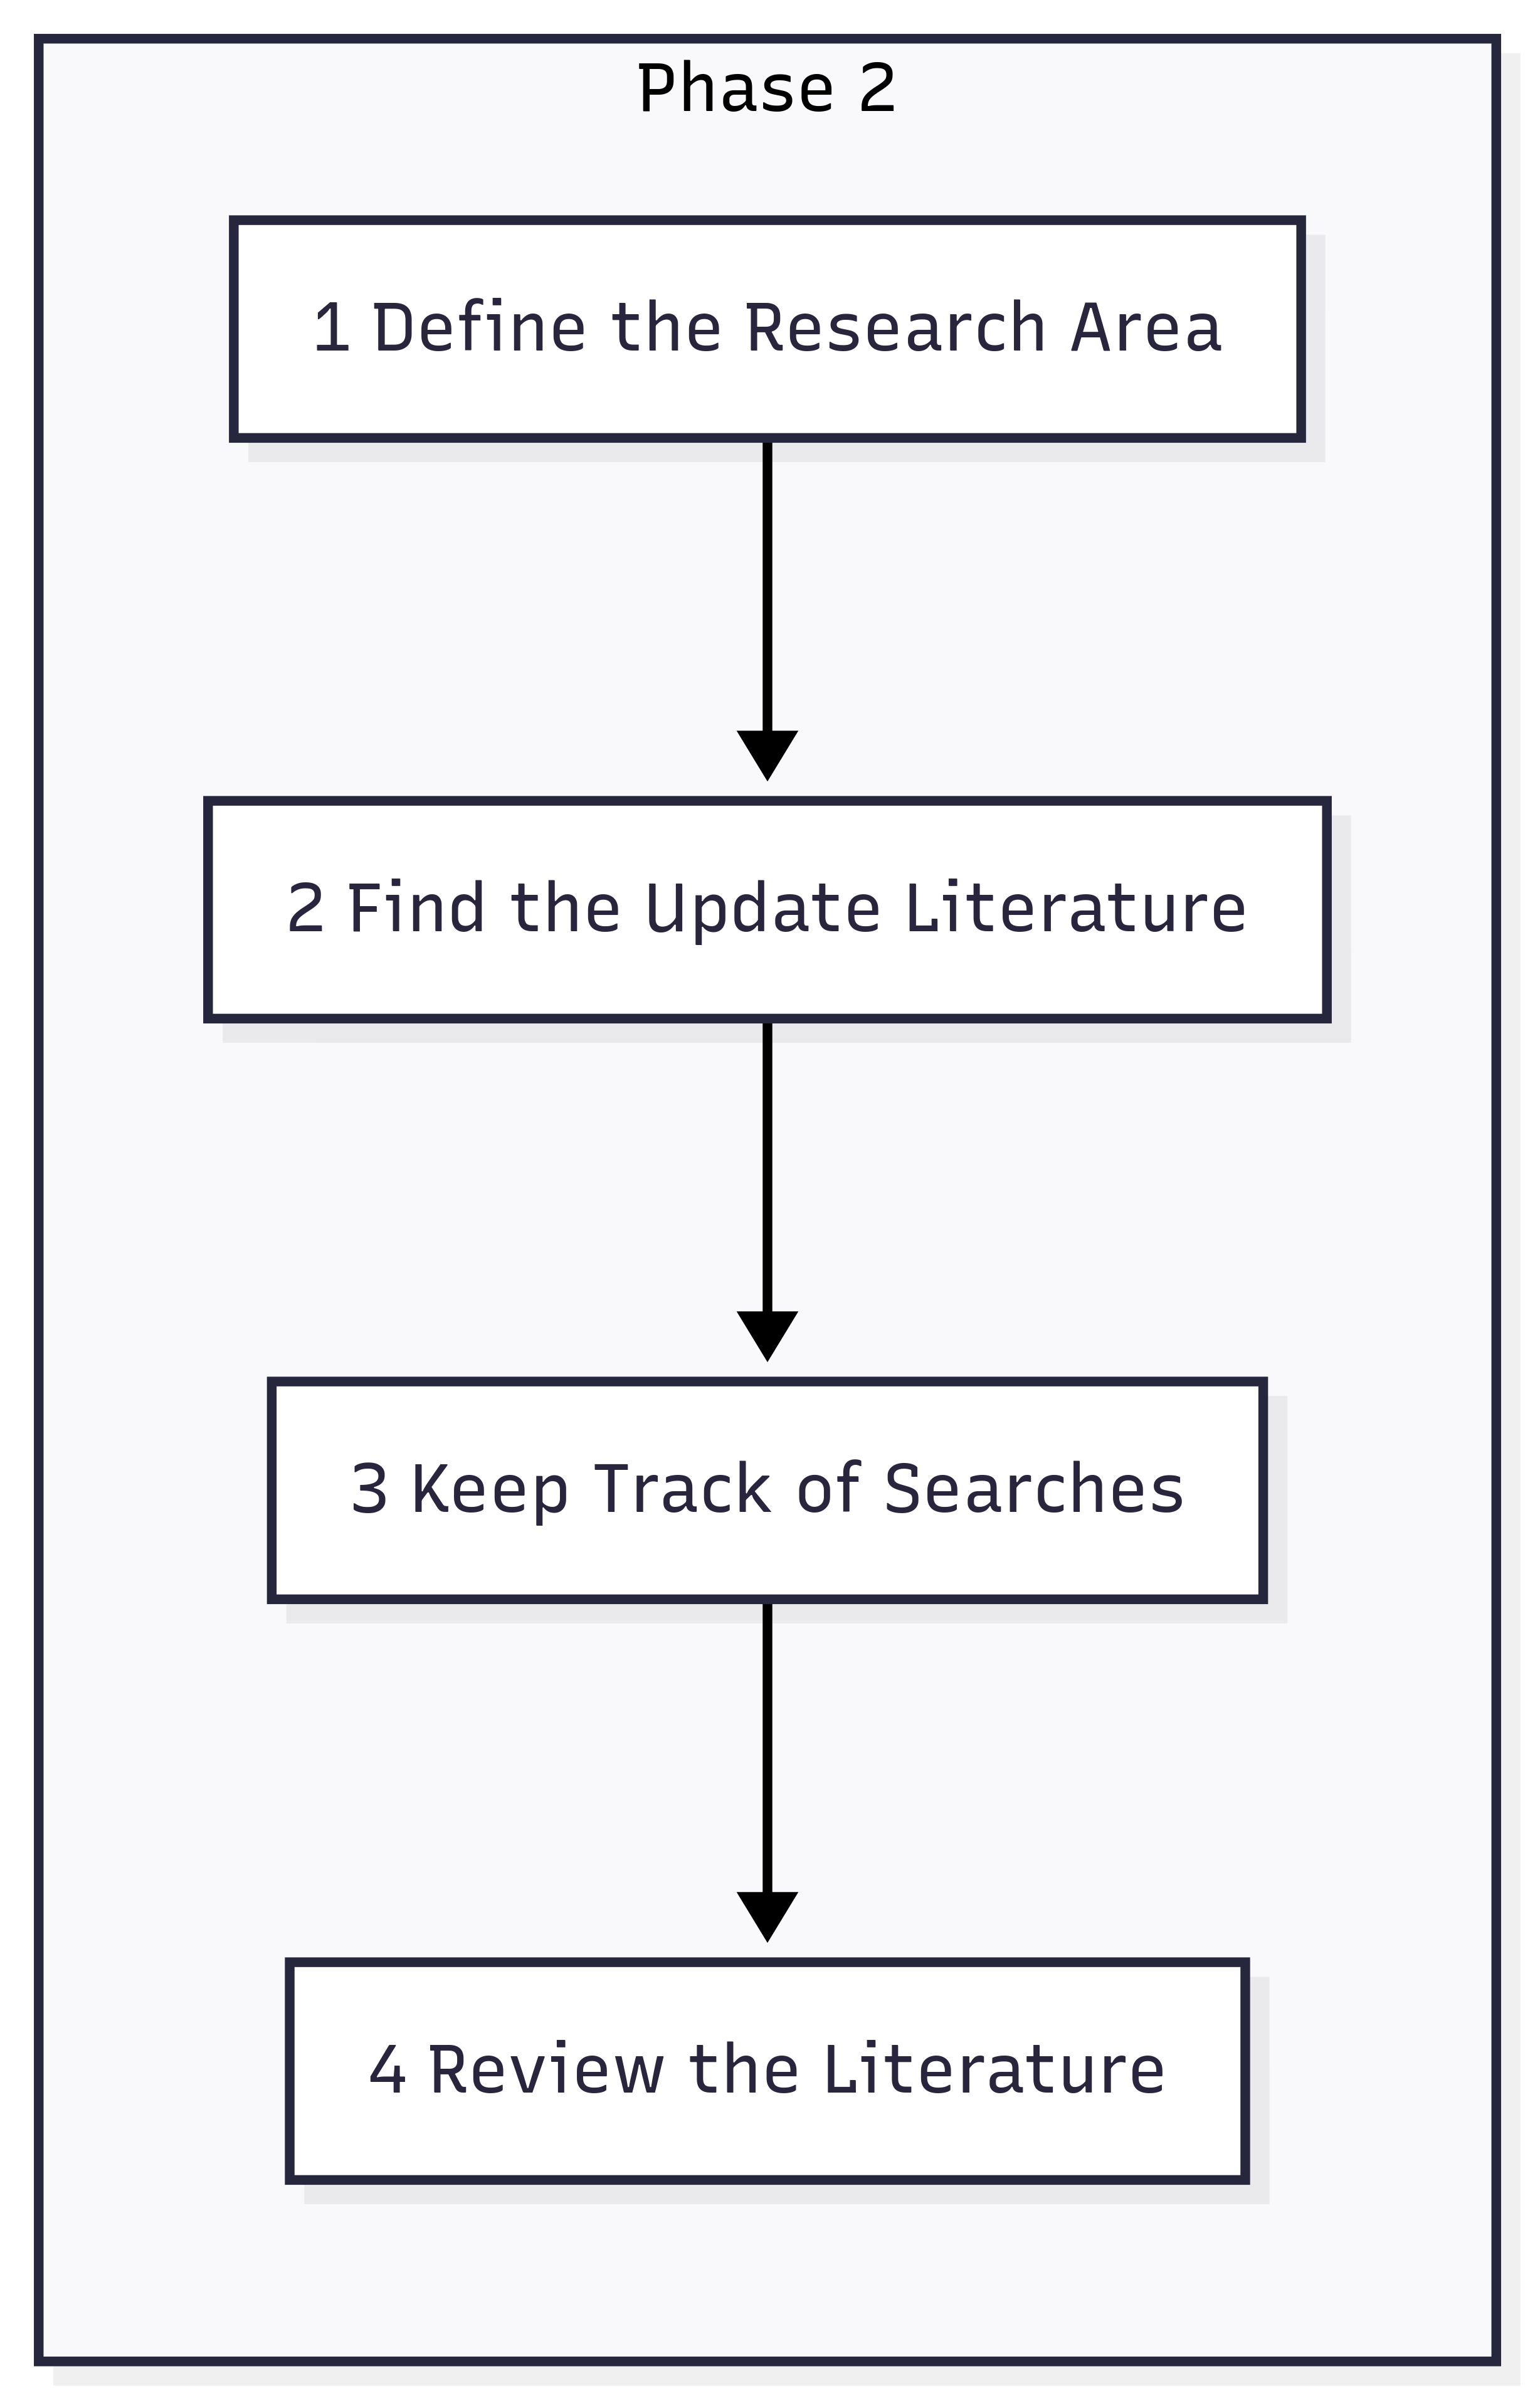
\includegraphics[height=14cm]{figure/framework-development-phase-2.png}
    \caption{Proactive Forensic Framework Development Phase 2}
    \label{fig:framework-development-phase-2}
\end{figure}
Figure~\ref{fig:framework-development-phase-2} presents Phase 2, which involves an extensive literature review to identify existing digital forensic frameworks, log management strategies, and relevant standards such as NIST SP 800-92. During this phase, the research area is scoped, updated literature is collected, search activity is recorded systematically, and selected works are critically analyzed. The aim is to extract best practices and determine the gaps the proposed framework should address.


\begin{figure}[H]
    \centering
    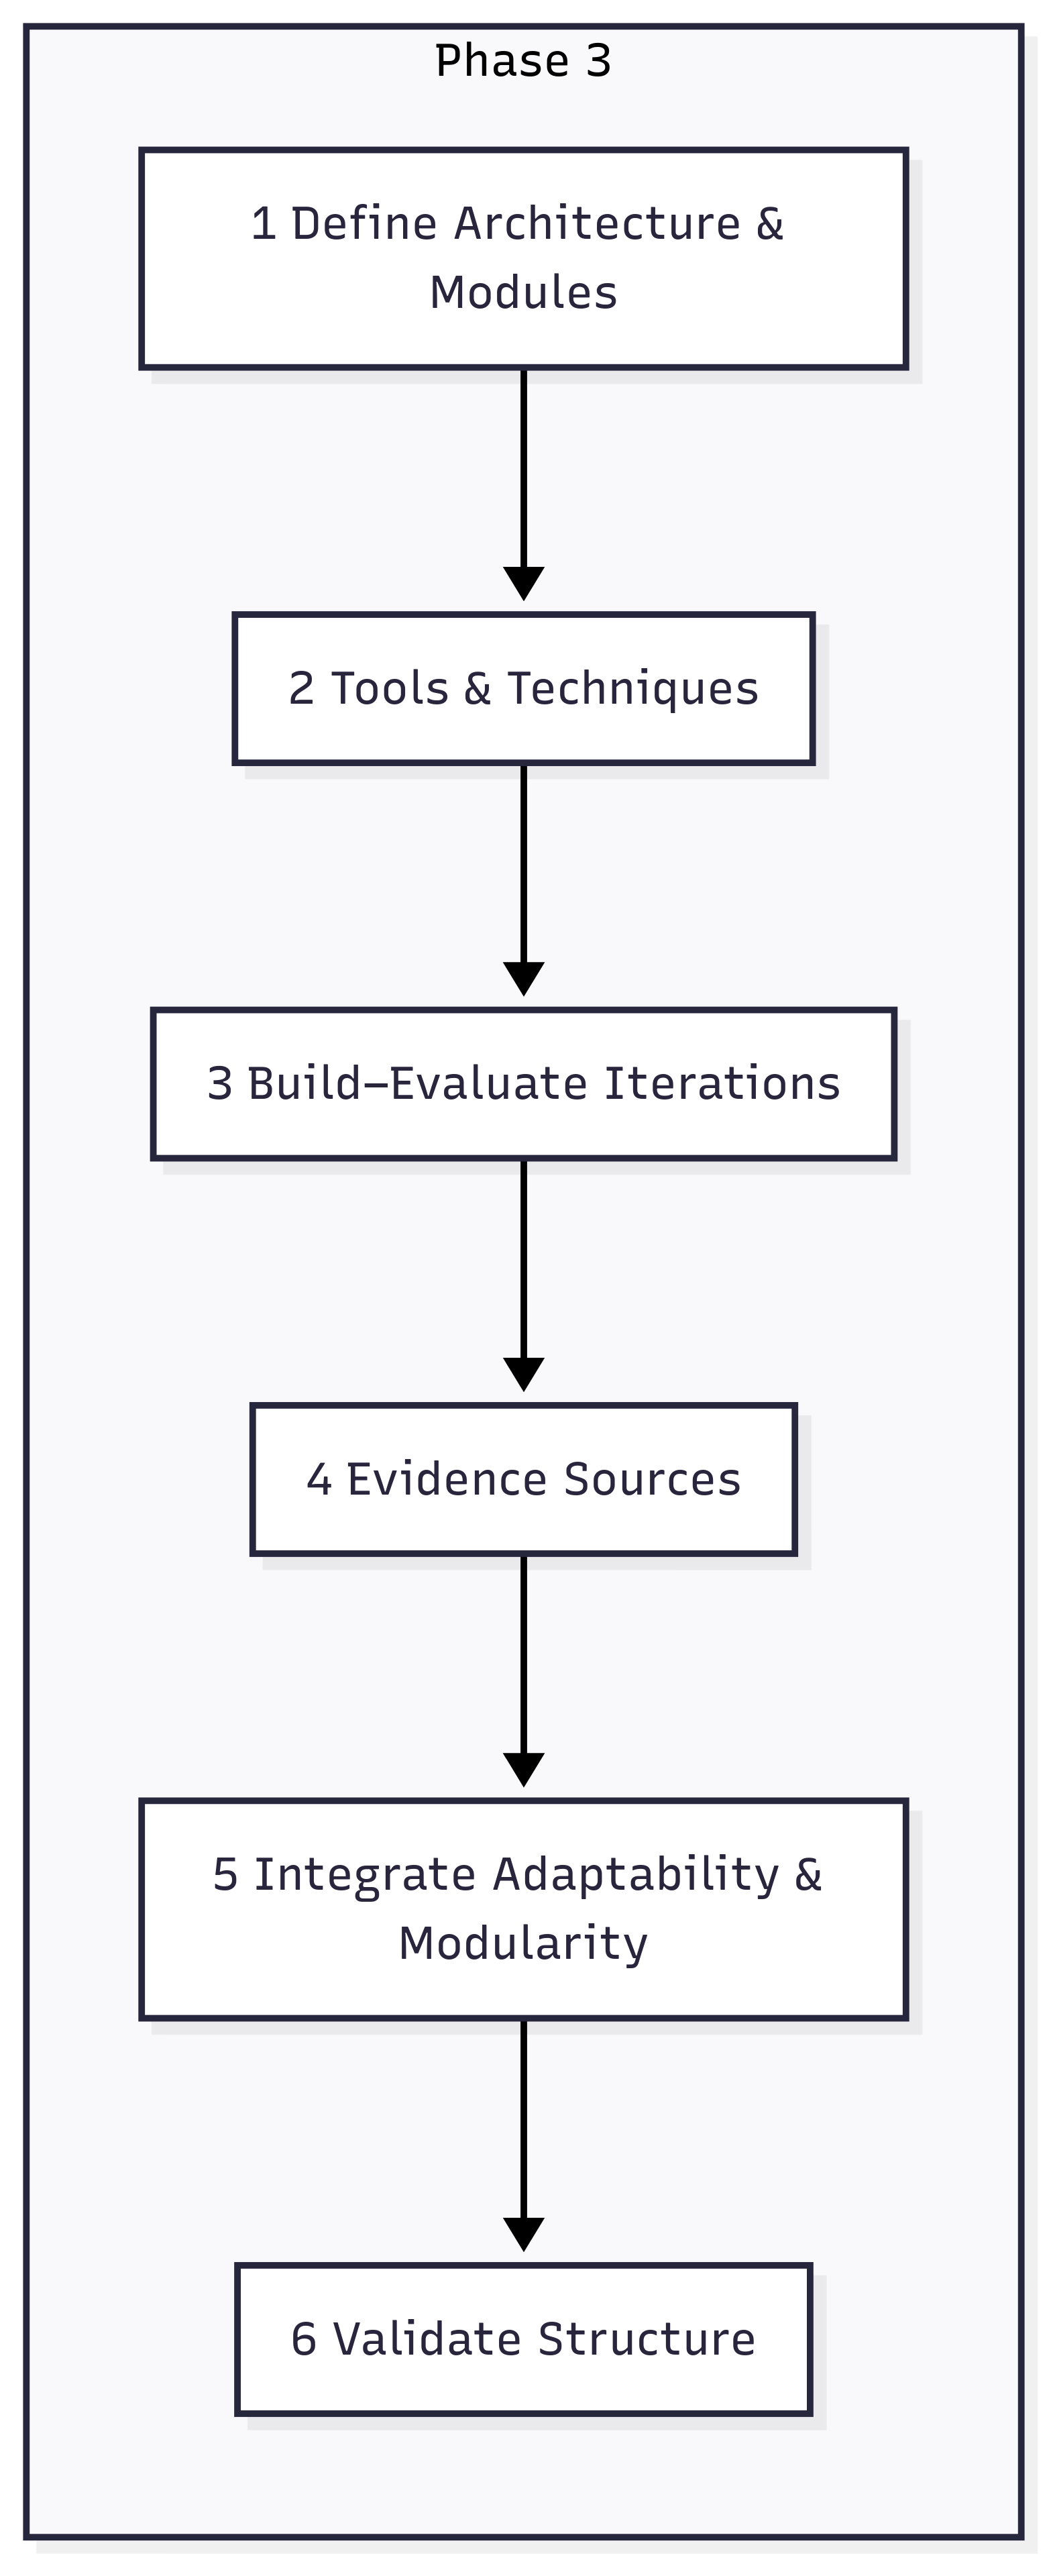
\includegraphics[height=14cm]{figure/framework-development-phase-3.png}
    \caption{Proactive Forensic Framework Development Phase 3}
    \label{fig:framework-development-phase-3}
\end{figure}
In Phase 3, illustrated in Figure~\ref{fig:framework-development-phase-3}, the framework architecture is designed and adapted based on the needs identified in earlier phases. The design follows a modular approach, integrating components such as log identification, proactive collection, transmission, analysis, and reporting. Each module is specified to align with proactive forensics goals, including real-time monitoring and traceability.


\begin{figure}[H]
    \centering
    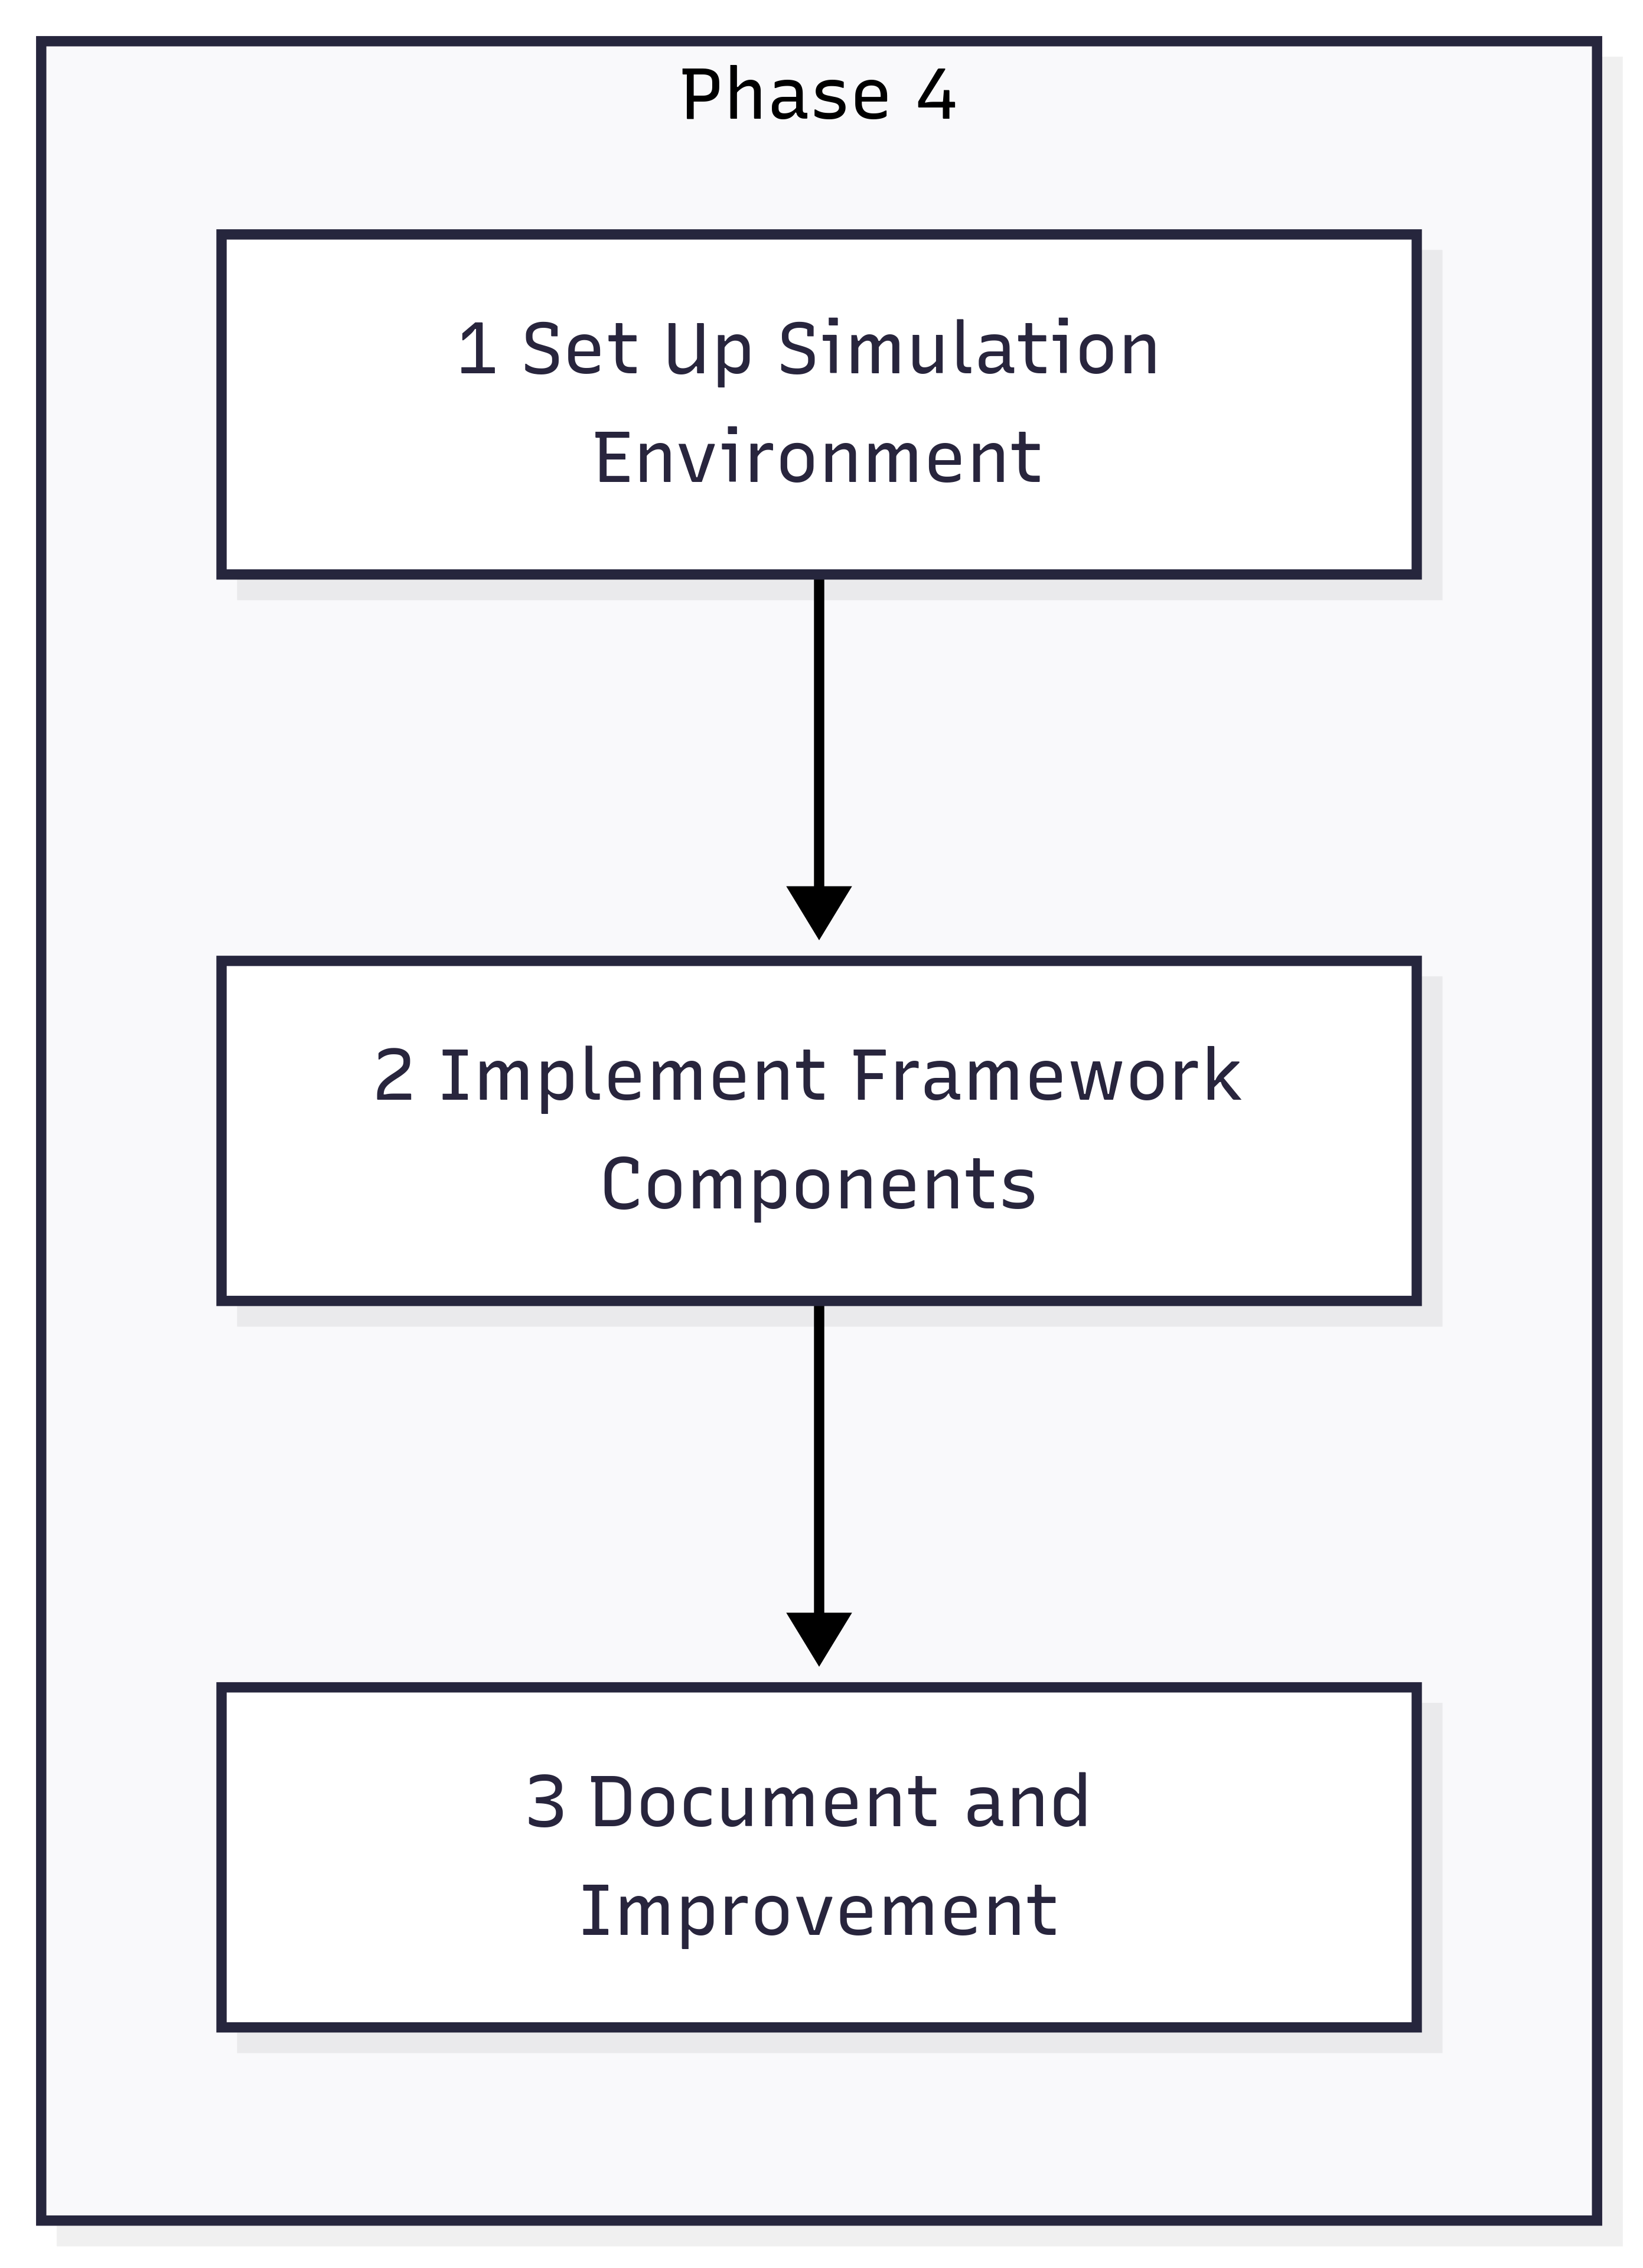
\includegraphics[height=14cm]{figure/framework-development-phase-4.png}
    \caption{Proactive Forensic Framework Development Phase 4}
    \label{fig:framework-development-phase-4}
\end{figure}

Figure~\ref{fig:framework-development-phase-4} details the implementation of the designed framework within a simulated environment. This phase includes configuring log sources, implementing data flow, integrating analysis tools, and simulating typical forensic scenarios (e.g., cheating attempts, unauthorized access). The prototype is developed iteratively, allowing for refinement based on observed results.


\begin{figure}[H]
    \centering
    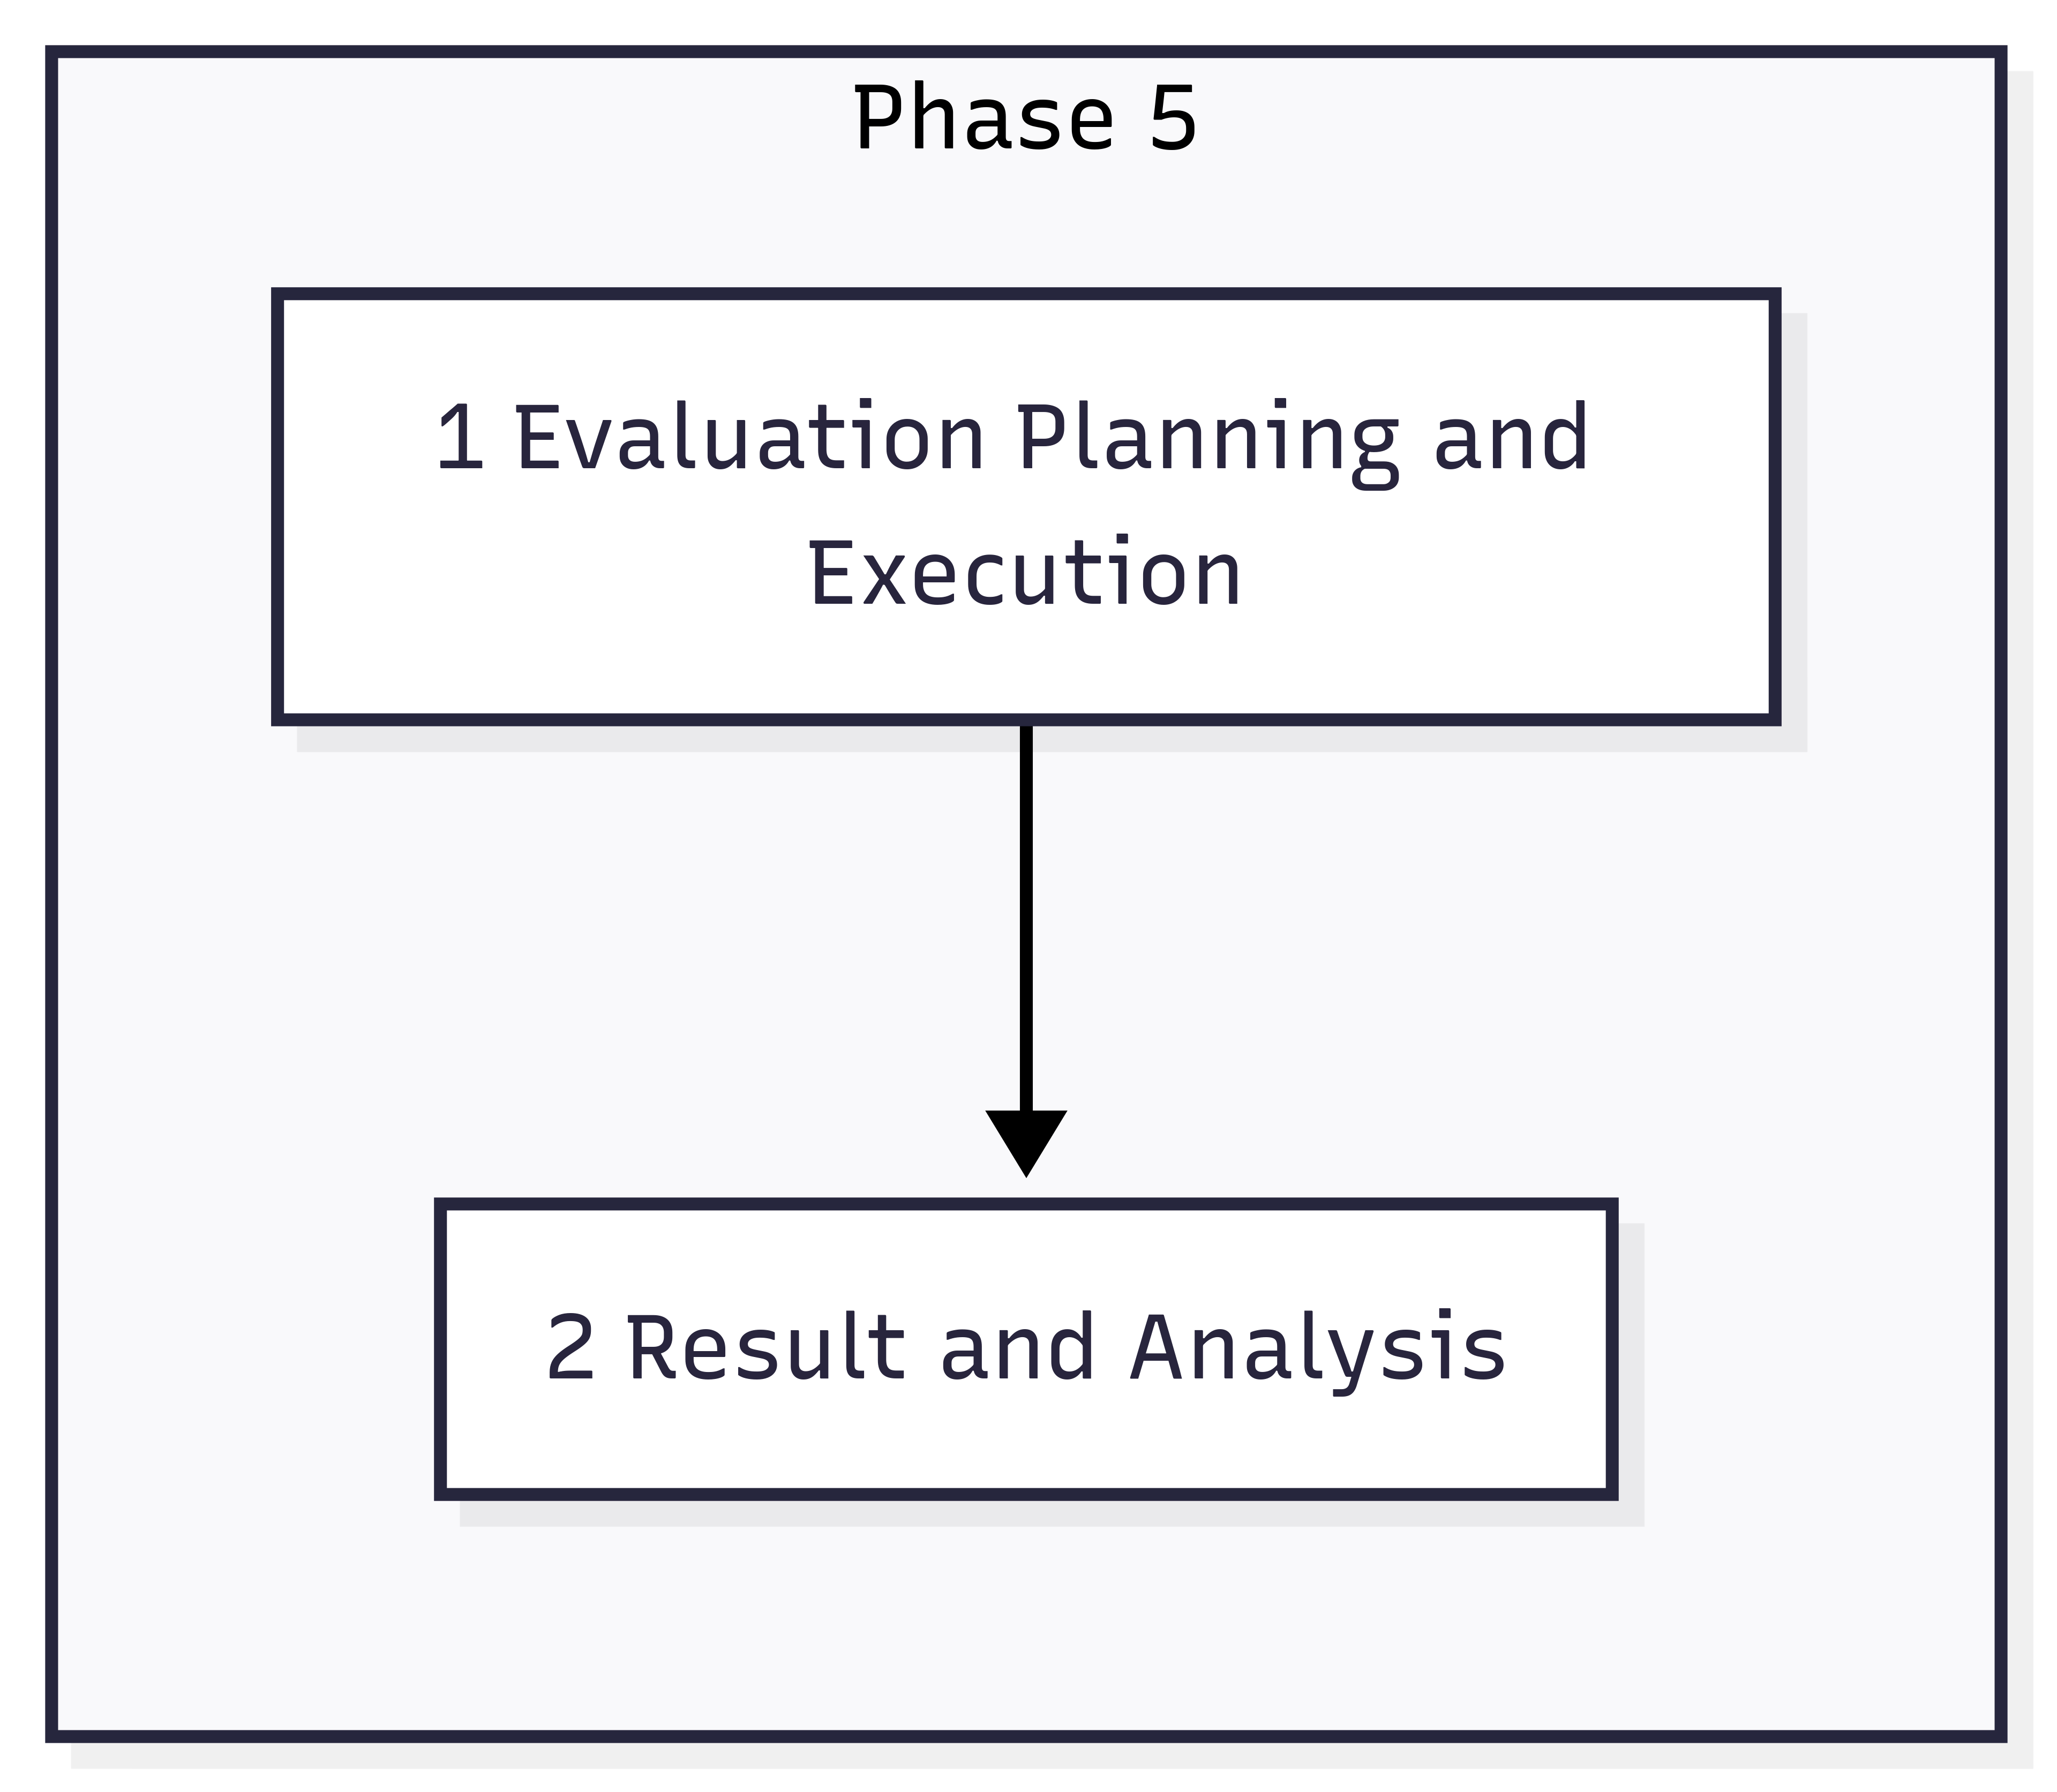
\includegraphics[height=14cm]{figure/framework-development-phase-5.png}
    \caption{Proactive Forensic Framework Development Phase 5}
    \label{fig:framework-development-phase-5}
\end{figure}

Figure~\ref{fig:framework-development-phase-5}, focuses on evaluating the framework using predefined metrics such as accuracy, timeliness, and detection capability. Experts from the digital forensic domain are engaged to validate the framework through structured interviews and feedback instruments. Their input helps verify the practical relevance and completeness of the framework, ensuring its applicability in real-world online education settings.

The evaluation phase follows a structured flow adapted from Marturana \textit{et al.}~\cite{marturana2020evaluation}, starting from the definition of metrics, followed by test design, controlled execution, result analysis, strength identification, and concluding with actionable recommendations.

\begin{figure}[H]
    \centering
    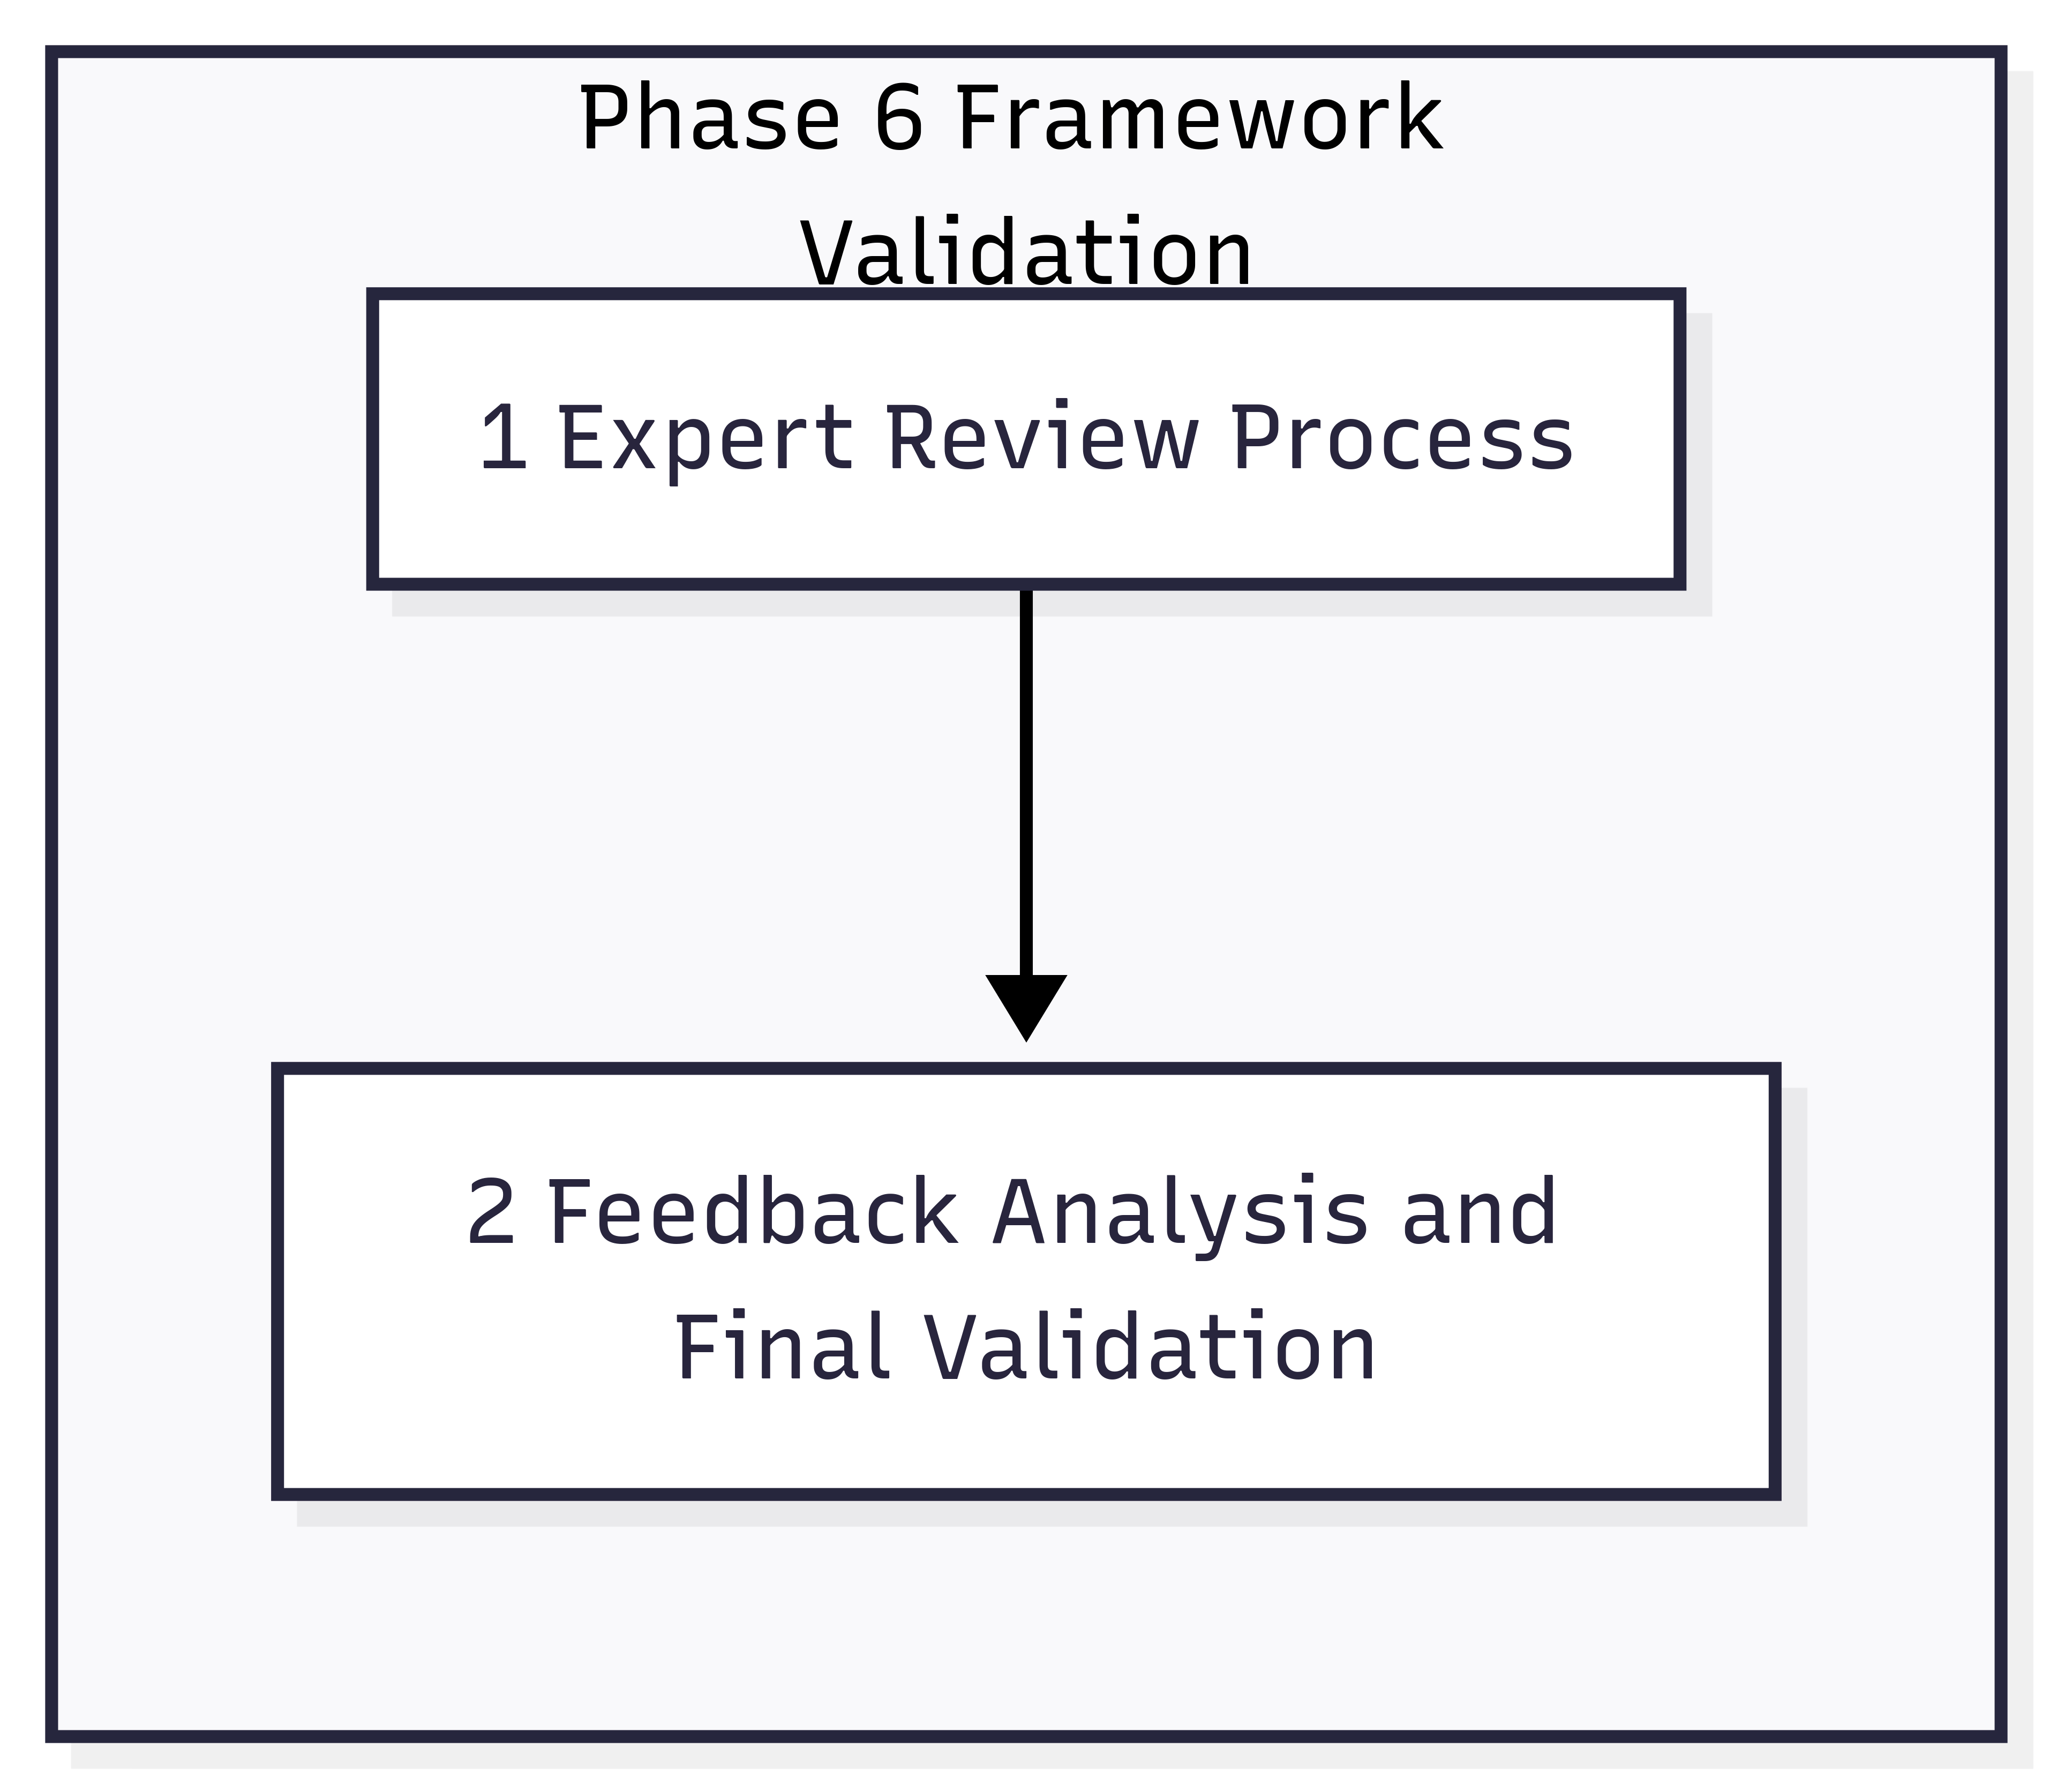
\includegraphics[height=14cm]{figure/framework-development-phase-6.png}
    \caption{Proactive Forensic Framework Development Phase 6}
    \label{fig:framework-development-phase-6}
\end{figure}

The final phase is as shown in Figure~\ref{fig:framework-development-phase-6}, the sixth phase involves validating the overall framework through expert evaluation. This phase is crucial to ensure the scientific, technical, and practical credibility of the framework. The process begins with identifying suitable experts in digital forensics, cybersecurity, and online education systems. A structured validation instrument—such as a questionnaire or interview protocol—is developed to guide the expert review.

Phase~6 sub-phases align with the Reliability Validation Enabling Framework (RVEF) proposed by \citet{stoykova2023rvef}, which defines a structured process to ensure forensic methods and tools are reliable across three tiers: technical, methodological, and applied~\cite{stoykova2023rvef}. RVEF mandates expert-based evaluation, instrumented testing, reliability analysis against standards, and formal documentation of outcomes — fully supporting sequential steps of identifying domain experts, preparing validation instruments, collecting expert reviews, analyzing feedback, confirming validity, and documenting enhancements.


\subsection{Log Management Implementation}

The implementation of the log management system is designed to support proactive forensic readiness within an online examination environment. The system consists of several key components that are integrated to enable automated log acquisition, secure storage, and effective analysis. The implementation follows the NIST 800-92 framework as a reference for security log management practices.

The main components of the implementation are as follows:

\begin{itemize}
    \item \textbf{Log Sources:} The system captures log data from multiple sources, including database logs (e.g., quiz attempts, login sessions), operating system logs, and application-level logs.

    \item \textbf{Log Collection:} A job scheduler is used to automate the periodic retrieval of log data. This ensures consistent and timely acquisition of relevant logs during and after exam sessions.

    \item \textbf{Log Transmission:} Collected logs are transmitted to a centralized storage server through secure channels. This step ensures all data is available for centralized processing and analysis.

    \item \textbf{Log Storage:} Logs are stored in a structured directory format with timestamping, access control, and checksum validation to ensure data integrity and traceability.

    \item \textbf{Log Analysis:} A dashboard interface is used to visualize log activity, while anomaly detection is performed using the Isolation Forest algorithm to identify suspicious patterns.

    \item \textbf{Alerting and Reporting:} The system provides real-time notifications for potential cheating incidents and generates structured PDF reports to support further forensic investigation.
\end{itemize}

This implementation ensures that log data is collected, preserved, and analyzed in a manner that supports digital forensic objectives, while also enabling timely administrative responses to security incidents during online examinations.
% \subsubsection{Log Source Identification}
% \subsubsection{Log Proactive Collection}
% \subsubsection{Log Transmission}
% \subsubsection{Log Storage}
% \subsubsection{Log Analysis}
% \subsubsection{Log Reporting}

\subsection{Log Management Testing Phase}

The testing phase aims to ensure that each process within the implemented log management system functions correctly and supports proactive digital forensic readiness, particularly in the context of online examinations. The evaluation is conducted sequentially, based on the nine log management processes previously defined. Each stage is tested using scenarios that simulate realistic conditions and are aligned with modeled threats, such as impersonation attacks (e.g., exam proxy or ``joki'') via remote access tools.

The testing stages are outlined as follows:

\begin{enumerate}
    \item \textbf{Log Identification Testing} \\
    Verifies that all log sources, including those from the exam platform, third-party applications, and operating systems, are successfully identified. The system should be capable of handling a variety of log formats, including those from legacy systems (e.g., plaintext, CSV).
    
    \item \textbf{Proactive Log Collection Testing} \\
    Ensures that log data is collected periodically through automated mechanisms. The system is tested under normal and high-load conditions to evaluate reliability and to identify potential performance bottlenecks.
    
    \item \textbf{Log Transmission Testing} \\
    Assesses the secure and timely transmission of log files from source systems to a centralized log server. The focus is on consistency, fault tolerance, and resistance to network delays or failures.
    
    \item \textbf{Log Storage Testing} \\
    Evaluates whether logs are stored in a structured and secure repository with appropriate access controls. Tests also verify retention policies and file integrity protection mechanisms.
    
    \item \textbf{Log Analyzer Testing} \\
    Confirms that the log analyzer or dashboard properly aggregates and displays data from various log formats. Usability and clarity of visualized user activity are key evaluation aspects.
    
    \item \textbf{Proactive Log Analysis Testing} \\
    Validates the system's capability to detect anomalies using machine learning techniques. Test data simulating both normal and suspicious behaviors is used to assess classification accuracy and anomaly detection effectiveness.
    
    \item \textbf{Notification Testing} \\
    Ensures that the system can generate and deliver alerts in response to detected suspicious activity. The testing includes verification of trigger conditions, content accuracy, and notification timeliness.
    
    \item \textbf{Log Preservation Testing} \\
    Verifies the system’s ability to export and preserve logs in a tamper-evident format using cryptographic checksums. File integrity checks are conducted to confirm that no modifications occur after export.
    
    \item \textbf{Log Reporting Testing} \\
    Confirms the ability of the system to generate readable and standardized reports summarizing user activity, typically in PDF format. The report structure and content relevance are evaluated.
\end{enumerate}

